\documentclass{article}
\usepackage{physics}
\usepackage{graphicx}
\usepackage{caption}
\usepackage{amsmath}
\usepackage{bm}
\usepackage{framed}
\usepackage{authblk}
\usepackage{empheq}
\usepackage{amsfonts}
\usepackage{esint}
\usepackage[makeroom]{cancel}
\usepackage{dsfont}
\usepackage{centernot}
\usepackage{mathtools}
\usepackage{subcaption}
\usepackage{bigints}
\usepackage{amsthm}
\theoremstyle{definition}
\newtheorem{lemma}{Lemma}
\newtheorem{defn}{Definition}[section]
\newtheorem{prop}{Proposition}[section]
\newtheorem{rmk}{Remark}[section]
\newtheorem{thm}{Theorem}[section]
\newtheorem{exmp}{Example}[section]
\newtheorem{prob}{Problem}[section]
\newtheorem{sln}{Solution}[section]
\newtheorem*{prob*}{Problem}
\newtheorem{exer}{Exercise}[section]
\newtheorem*{exer*}{Exercise}
\newtheorem*{sln*}{Solution}
\usepackage{empheq}
\usepackage{tensor}
\usepackage{xcolor}
%\definecolor{colby}{rgb}{0.0, 0.0, 0.5}
\definecolor{MIT}{RGB}{163, 31, 52}
\usepackage[pdftex]{hyperref}
%\hypersetup{colorlinks,urlcolor=colby}
\hypersetup{colorlinks,linkcolor={MIT},citecolor={MIT},urlcolor={MIT}}  
\usepackage[left=1in,right=1in,top=1in,bottom=1in]{geometry}
\usepackage{newpxtext,newpxmath}
\newcommand*\widefbox[1]{\fbox{\hspace{2em}#1\hspace{2em}}}
\newcommand{\p}{\partial}
\newcommand{\R}{\mathbb{R}}
\newcommand{\C}{\mathbb{C}}
\newcommand{\lag}{\mathcal{L}}
\newcommand{\nn}{\nonumber}
\newcommand{\ham}{\mathcal{H}}
\newcommand{\M}{\mathcal{M}}
\newcommand{\I}{\mathcal{I}}
\newcommand{\K}{\mathcal{K}}
\newcommand{\F}{\mathcal{F}}
\newcommand{\w}{\omega}
\newcommand{\lam}{\lambda}
\newcommand{\al}{\alpha}
\newcommand{\be}{\beta}
\newcommand{\x}{\xi}
\newcommand{\G}{\mathcal{G}}
\newcommand{\f}[2]{\frac{#1}{#2}}
\newcommand{\ift}{\infty}
\newcommand{\lp}{\left(}
\newcommand{\rp}{\right)}
\newcommand{\lb}{\left[}
\newcommand{\rb}{\right]}
\newcommand{\lc}{\left\{}
\newcommand{\rc}{\right\}}
\newcommand{\V}{\mathbf{V}}
\newcommand{\U}{\mathcal{U}}
\newcommand{\Id}{\mathcal{I}}
\newcommand{\D}{\mathcal{D}}
\newcommand{\Z}{\mathcal{Z}}

%\setcounter{chapter}{-1}

\usepackage{enumitem}
\usepackage{listings}
\captionsetup[lstlisting]{margin=0cm,format=hang,font=small,format=plain,labelfont={bf,up},textfont={it}}
\renewcommand*{\lstlistingname}{Code \textcolor{violet}{\textsl{Mathematica}}}
\definecolor{gris245}{RGB}{245,245,245}
\definecolor{olive}{RGB}{50,140,50}
\definecolor{brun}{RGB}{175,100,80}

%\hypersetup{colorlinks,urlcolor=colby}
\lstset{
	tabsize=4,
	frame=single,
	language=mathematica,
	basicstyle=\scriptsize\ttfamily,
	keywordstyle=\color{black},
	backgroundcolor=\color{gris245},
	commentstyle=\color{gray},
	showstringspaces=false,
	emph={
		r1,
		r2,
		epsilon,epsilon_,
		Newton,Newton_
	},emphstyle={\color{olive}},
	emph={[2]
		L,
		CouleurCourbe,
		PotentielEffectif,
		IdCourbe,
		Courbe
	},emphstyle={[2]\color{blue}},
	emph={[3]r,r_,n,n_},emphstyle={[3]\color{magenta}}
}

\begin{document}

\begin{center}
	\Large{The lineshape of RF association of Feshbach molecules}
\end{center}	
	
\begin{center}
	\large{Huan Q. Bui}
\end{center}

\begin{center}
	\today
\end{center}

\section{Context}

We consider the free-to-bound transition: an rf photon associates two free atom into a (weakly-bound) Feshbach molecule. The lineshape can be obtained from Fermi's Golden rule: it is a product of the Franck-Condon overlap $\mathcal{F}$ between the wavefunction of a bound Feshbach molecule and that of a pair of two free atoms and the probability $p$ of finding two free atoms in phase space which, along with the RF photon, satisfy the required resonance condition.

\section{Franck-Condon factor calculation}

Here we follow the steps outlined by \cite{FB_rf_1}. We first provide the bound and free wavefunctions. The normalized molecule wavefunction is assumed to have the typical asymptotic form:
\begin{equation}
\phi_m = \sqrt{\f{2}{a}}\f{\exp(-r/a)}{r}
\end{equation}
where $a$ is the scattering length which, along with the background scattering length $a_{bg}$, gives the binding energy $E_b = \hbar^2 / 2\mu (a - \overline{a})^2$, where $\overline{a}$ is the mean scattering length. The free atom pair assumes a scattering wavefunction $\psi_k(r) \propto \sin(kr + \delta') / r$, where $k$ is the wavevector associated with the kinetic energy $E_k = \hbar^2 k^2 / 2\mu$ of the incoming wave and $\delta'$ is the phase-shift associated with the scattering length $a' = a_{bg}$ of the free-atom pair. While wavefunctions of scattering states are not normalizable in the usual sense, they are $\delta$-function normalizable. We first follow \cite{FB_rf_1} and require that the scattering wavefunctions be energy-normalized:
\begin{equation}
\int \psi_k(r)^* \psi_{k'}(r)r^2 \,dr = \pi \delta(E_k-E_k') = \delta(k-k') \f{ \pi \hbar^2 k}{2\mu},
\end{equation}
where the second equality comes from the composition rule for the $\delta$-function. From here, we find the appropriate normalization:
\begin{equation}
\psi_k(r) = \sqrt{\f{2\mu}{\pi\hbar^2 k}} \f{\sin(kr + \delta')}{r}.
\end{equation}
The Franck-Condon overlap can now be evaluated:
\begin{equation}\label{eq:FC}
\mathcal{F}(k)= \abs{\int_0^\infty \phi_m^*(r) \psi_k(r)r^2 \,dr}^2 =   \f{4a \mu (a k \cos\delta' + \sin \delta')^2}{\pi \hbar^2 k (1 + a^2 k^2)^2}. 
\end{equation}
\noindent 
The interaction range $r_0$ for the Van der Waals potential of $^{23}$Na and $^{40}$K is given by 
\begin{equation}
r_0 = 2^{-3/2} \f{\Gamma(3/4)}{\Gamma(5/4)} \lp \f{2\mu C_6}{\hbar^2} \rp^{1/4} \approx 50 a_0,
\end{equation}
where $C_6 \approx 2322 \, E_\text{Hartree} \, a_0^6\footnote{need citation, see Tiecke 2010}$. In the Fermi1 experiment, $T \approx 200 \text{ nK}$, so $k \sim \sqrt{2 \mu k_B T / \hbar^2} \approx 1 / 6000 a_0 \ll 1/r_0 = 1/ 50 a_0$. As a result, we may use the low-energy expansion of the scattering phase shift:
\begin{equation}
k \cot \delta' \approx - \f{1}{a'} + \f{r_e'}{2} k^2 + \mathcal{O}(k^4) \approx -\f{1}{a'} = -\f{1}{a_{bg}}
\end{equation}
where $r_e' = \Gamma(1/4)^4 r_0 / 6\pi^2$. Substituting this into Eq. \eqref{eq:FC}, we find 
\begin{equation*}
\mathcal{F}(k) = \f{4 a (a - a_{bg})^2 k \mu }{\pi \hbar^2 (1 + a^2 k^2 )^2  (1 + a^2_{bg} k^2 )}.
\end{equation*}

\section{Calculating the probability of finding a suitable pair of atoms for Feshbach RF association}

Consider a particle in a 3D harmonic trap. The Hamiltonian is 
\begin{equation}
\ham(\mathbf{p}, \mathbf{r}) = \f{\mathbf{p}^2}{2m} + \f{1}{2} \sum_i^3 m\omega_i^2 \mathbf{r}_i^2.
\end{equation}
The probability of finding the particle in some phase space cell $d^3\mathbf{p} d^3 \mathbf{r}$ at temperature $T$ is given by 
\begin{equation}
\Pr(\mathbf{p}, \mathbf{r}) = \frac{1}{\mathcal{Z}} \exp\lp -\be\ham \rp = \f{\exp(-\be \ham)}{\int d^3 p \int d^3 r \exp (-\be \ham) } = \f{\overline{\omega}^3}{(2\pi k_BT)^3} \exp(\ham / k_BT))
\end{equation}
where $\be = k_BT$ and $\overline{\omega}$ denotes the geometric mean of the three trapping frequencies. \\

\noindent Now let us introduce another particle. Let these two particles be an Na atom and a K atom and assume that they do not interact. The probability for finding them textit{somewhere} in phase space is trivially the product $\Pr(\mathbf{p}_\text{Na}, \mathbf{r}_\text{Na}) \times \Pr(\mathbf{p}_\text{K}, \mathbf{r}_\text{K})$. For RF association, we are interested in the total probability of finding a pair of Na and K for which their \textit{relative kinetic energy} and the RF photon energy satisfy the energy conservation condition for molecular association:
\begin{equation}
E_k = \f{\hbar^2 k^2}{2\mu} = \hbar \omega - E_b,
\end{equation}
where $\mu$ is the reduced mass $m_\text{Na} m_\text{K} / (m_\text{Na} + m_\text{K})$. In order to define $E_k$ and evaluate the total probability of finding an Na and a K atom that satisfy this condition, we must first transform to the COM and reduced mass coordinates. The COM and relative coordinates are given by
\begin{equation}
\mathbf{r}_\text{COM} = \f{m_\text{Na} \mathbf{r}_\text{Na} + m_\text{K} \mathbf{r}_\text{K}}{ m_\text{Na} + m_\text{K}},
\quad\quad 
\mathbf{r}_\text{rel} = \mathbf{r}_\text{K}  - \mathbf{r}_\text{Na}, 
\quad\quad
M = m_\text{Na} + m_\text{K},
\quad\quad 
\mu = \f{m_\text{Na} m_\text{K} }{m_\text{Na} + m_\text{K}}
\end{equation}
from which it follows that
\begin{eqnarray}
\ham &=&  \f{\mathbf{p}_\text{Na}^2}{2m_\text{Na}} + \f{\mathbf{p}_\text{K}^2}{2m_\text{K}} + 
\underbrace{\f{1}{2} \sum_i^3 m_\text{Na}\omega_{i,\text{Na}}^2 \mathbf{r}_{i,\text{Na}}^2 + \f{1}{2} \sum_i^3 m_\text{K}\omega_{i,\text{K}}^2 \mathbf{r}_{i,\text{K}}^2} \\ 
&=& \f{\mathbf{p}_\text{COM}^2}{2M} + \f{\mathbf{p}^2_\text{rel}}{2\mu}  + V( \mathbf{r}_\text{Na}, \mathbf{r}_\text{K} )
\end{eqnarray}
where the relative term is simply the sum of the kinetic energies calculated relative to the COM:
\begin{equation}
\f{1}{2}m_\text{Na}(\dot{\mathbf{r}}_\text{Na} - \dot{r}_\text{COM})^2 + \f{1}{2}m_\text{K}(\dot{\mathbf{r}}_\text{K} - \dot{r}_\text{COM})^2 = \f{1}{2} \f{m_\text{Na}m_\text{K}}{m_\text{Na} + m_\text{K}} (\dot{\mathbf{r}}_\text{K}  - \dot{\mathbf{r}}_\text{Na} )^2 \equiv \f{\mathbf{p}_\text{rel}^2}{2\mu}.
\end{equation}
Here, we have defined $\mathbf{p}_\text{rel} \equiv \mu \dot{\mathbf{r}}_\text{rel}$. Additionally, we have assumed that $\omega_{i,\text{Na}} = \omega_{i,\text{K}} = \omega_i$ for all $i = x,y,z$. We note that is a fairly safe assumption to make, since $\omega_\text{K} / \omega_\text{Na} \approx 1.16$ in reality. \\

\noindent The probability of finding a pair of Na and K atoms with $E_k = \hbar \omega - E_b$ is a product of the spatial and momentum integrals. These are uncoupled, so we can evaluate them separately. With overall normalization factor, the spatial integrals give the contribution
\begin{equation}
S = \f{(2\pi k_BT)^3}{(m_\text{Na} m_\text{K})^{3} \overline{\omega}^6} \times \lp \f{\overline{\omega}}{2\pi k_B T} \rp^6 = \f{1}{(2\pi k_BT)^3} \f{1}{(m_\text{Na} m _\text{K})^{3}}.
\end{equation}
The momentum integral has two uncoupled parts: the COM integral and relative integral. The Jacobian for the  $(\mathbf{p}_\text{Na}, \mathbf{p}_\text{K}) \to (\mathbf{p}_\text{COM}, \mathbf{p}_\text{rel})$ is unity. The COM integral reads:
\begin{equation}
M_\text{COM} = (2 \pi M k_BT)^{3/2}.
\end{equation}
The integral involving the relative kinetic energy is a convolution of the "bare" relative kinetic energy and a $\delta$-function for picking out the correct kinetic energy:
\begin{eqnarray}
M_\text{rel} 
&=& \int d^3 p_\text{rel} \exp\lp -p^2_\text{rel}/2 \mu \rp \delta\lp p_\text{rel}^2 / 2\mu = E_k  \rp \\
&=& \int d^3 p_\text{rel} \exp\lp -p^2_\text{rel}/2 \mu \rp \delta\lp p_\text{rel}^2 / 2\mu = E_k  \rp \\
&=& \int d^3 p_\text{rel} \exp\lp -p^2_\text{rel}/2 \mu \rp \f{\mu}{\hbar k} \delta(p_\text{rel} = \hbar k)\\
&=& \f{4\pi \mu}{\hbar k} (\hbar k)^2  \exp\lp \f{-E_k}{k_BT} \rp\\
&=& 4\pi \mu \hbar k  \exp\lp \f{-\hbar^2 k^2}{2\mu k_B T} \rp.
\end{eqnarray}
Putting everything together, we find the desired expression for the probability of finding an Na-K pair satisfying the energy conservation condition:
\begin{equation}
\Pr(k) \propto \f{k}{(2\pi k_B T)^{3/2}} \exp \lp \f{-\hbar^2 k^2 }{2 \mu k_B T} \rp,
\end{equation}
where we have left out the irrelevant multiplicative constants and kept only factors that depend on the temperature $T$ and wavevector $k$. 

\section{The ideal lineshape}

From the previous two sections, we readily find the RF lineshape:
\begin{equation}
\Gamma(k) \propto \f{k}{(2\pi k_B T)^{3/2}} \exp \lp \f{-\hbar^2 k^2 }{2 \mu k_B T} \rp \times \f{4 a (a - a_{bg})^2 k \mu }{\pi \hbar^2 (1 + a^2 k^2 )^2  (1 + a^2_{bg} k^2 )}.
\end{equation}
With $k = \sqrt{2\mu (\hbar \omega - E_b) / \hbar^2 }$, we find 
\begin{equation}
\Gamma(\omega) \propto \f{\hbar \omega - E_b}{(k_BT)^{3/2}}  \f{1 }{\lb 1 + \f{2\mu a^2}{\hbar^2} (\hbar \omega - E_b) \rb^2  \lb 1 + \f{2\mu a_{bg}^2}{\hbar^2}  (\hbar \omega - E_b) \rb} \exp\lb \f{-(\hbar \omega - E_b)}{k_B T} \rb.
\end{equation}

For the purpose of fitting to RF lines, we care about the lineshape, which includes the "resonance" feature and its width. As a result, a more practical expression for the lineshape is as follows:
\begin{equation}
\Gamma(\omega) \propto 
\f{\omega - \omega_b}{\lp 1 + \f{\omega - \omega_b}{ \omega_a} \rp^2 \lp 1 + \f{\omega - \omega_b}{\omega_{a_{bg}}} \rp} 
\exp\lp -\f{\omega - \omega_b}{k_B T / \hbar } \rp. 
\end{equation}
What does this lineshape look like for some practical cases? Suppose we have $\omega_b = 2\pi \times 300 \text{ kHz}, \omega_a = 2\pi \times 287  \text{ kHz}, \omega_{a_{bg}} =  2\pi \times 259 \text{ kHz}$ and $T = 200$ nK $\implies k_BT / \hbar  = $. Then the lineshape looks something like the following.
\begin{figure}[!htb]
\centering
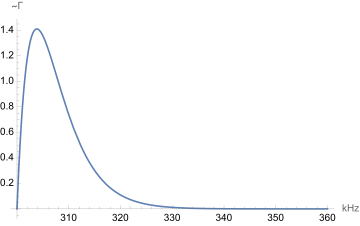
\includegraphics[scale = 1.0]{lineshape.eps}
\end{figure}


\section{Thermal equilibrium}


\section{Others}








\bibliography{FB_rf_association} 
\bibliographystyle{unsrt}	

\end{document}